\documentclass{article}
\usepackage{graphicx} % Required for inserting images
\usepackage{float}

\title{Tarea 3: LATEX}
\author{César Edahi Guajardo Barreto}
\date{ 22 de Septiembre 20
26}

\begin{document}

\maketitle

\section{¿Porqué deberías leer \textbf{\textit{"Dungeon Crawler Carl"}}?}
Dungeon Crawler Carl es una serie de libros del género LitRPG, esto significa que en este género los personajes actúan bajo la lógica de un juego RPG, es decir, ganan niveles, usan magia, tienen misiones, etc. Si alguna vez jugaste Skyrim sabrás exactamente a lo que me refiero.

Una vez establecido el marco de como funciona la historia, ¿De qué trata esta serie de libros?:

En el lejano tiempo de 2020, \textbf{\textit{Carl}} es un ex miembro de la guardia costera viviendo en Seattle, su vida es de lo más común para un estadounidense blanco, tiene un departamento modesto en la ciudad y un trabajo como mecánico de botes que no le desagrada. Vive con su novia y con su gato de raza persa, llamada \textbf{\textit{Princess Donut}}.

Una madrugada especialmente fría y nevada de invierno,  Carl se encuentra buscando departamentos en renta, su novia Beatrice acaba de subir una historia a sus redes en las que es más que obvio que esta con otro hombre y Carl ha decidido terminar la relación. En esos momentos Princess Donut salta por la ventana del departamento a un árbol cercano, Carl suspira y decide salir a rescatarla, y aprovechar para fumar un cigarro, decide que no vale la pena vestirse completamente solo para salir un momento y sale en boxers y crocs para rescatar a la gata de su reciente ex-novia.

Momentos después Carl se encuentra debajo del árbol, intentando tentar a la gata para que baje y puedan salir del fŕio los dos, en ese insante escucha un estruendo apocalíptico, al voltearse puede ver que su complejo departamental ha sido completamente aplanado, junto con cualquier edificio que alcance a ver. Una voz suena directamente en su cabeza: \textit{"Se notifica a la humanidad que el planeta Tierra ha sido oficialmente "recolectada" según la legislación del Sindicato Galáctico, dado que la civilización humana no logró desarrollar tecnología de viaje más rápido que la luz (FTL) ni registrar su soberanía a tiempo..."} , básicamente la tierra ha sido conquistada por una civilización multi-especie alienígena y escudada con legalismos vacíos han tomado control de la tierra y sus recursos. Este sindicato le da dos opciones a los sobrevivientes de la primera recolección: Sobrevive en la superficie del planeta por tus propios medios o participa en un evento conocido como \textbf{\textit{"The Crawl"}}, este evento consiste en un calabozo en donde los "crawlers" tendrán que sobrevivir diferentes niveles, con diferentes temáticas, con magia, diferentes razas fantásticas y todo bajo la batuta de una \textbf{\textit{IA}} inestable,todopoderosa y con fetiche por los \textbf{\textit{pies}} que funciona como \textbf{\textit{Dungeon Master}}.

Carl al no querer morir de hipotermia con el gato que ahora es suyo, decide entrar y probar sus suerte...

Estos son los títulos de los libros hasta el momento:

\begin{itemize}
\item Dungeon Crawler Carl

\item Carl's Doomsday Scenario

\item The Dungeon Anarchist's Cookbook

\item The Gate of the Feral Gods

\item The Butcher's Masquerade

\item The Eye of the Bedlam Bride

\item This Inevitable Ruin
\end{itemize}




\begin{figure}
    \centering
    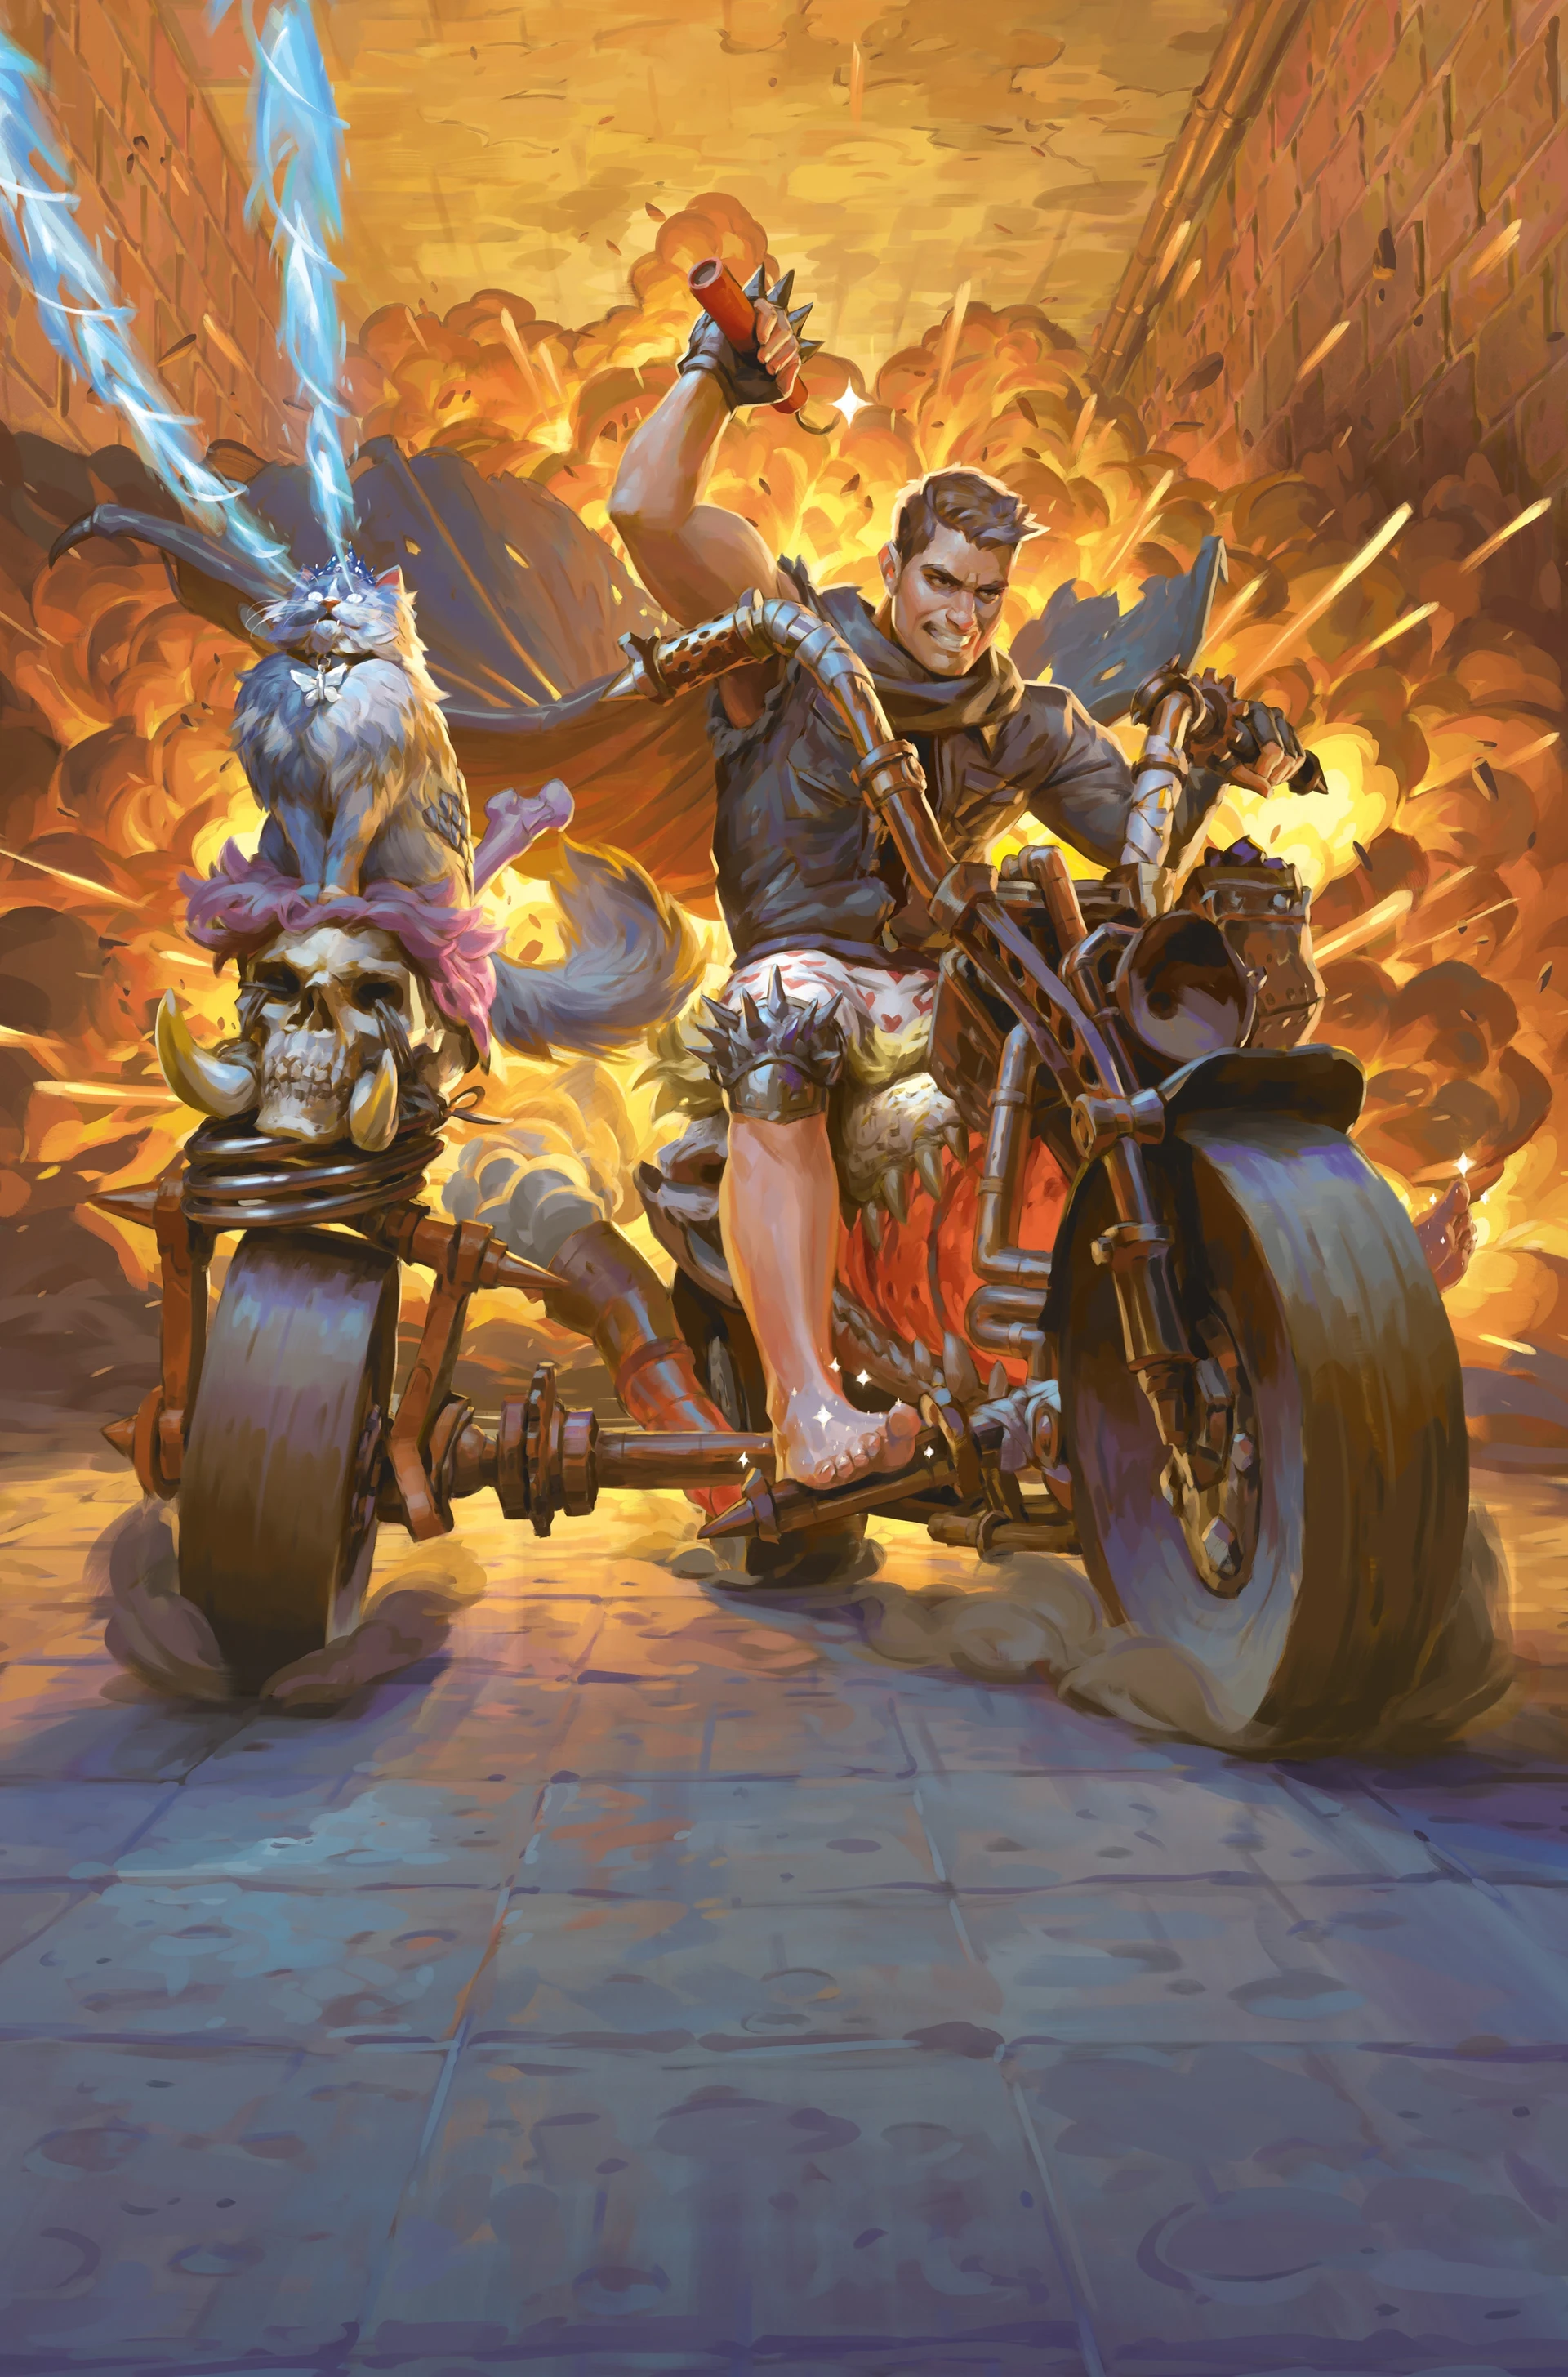
\includegraphics[width=0.75\linewidth]{image.png}
    \caption{Carl y Donut}
    \label{fig:placeholder}
\end{figure}



\end{document}
